\documentclass[twocolumn,showpacs,pre,preprintnumbers,floatfix]{revtex4-1}
\usepackage{graphicx}
\usepackage[english]{babel}
\usepackage{amssymb}
\usepackage{amsbsy}
\usepackage{amsmath}
\usepackage{color}
\usepackage{natbib}
\usepackage{tikz,pgfplots}
\usetikzlibrary{spy}

\newcommand{\todo}[1]{ \fbox{{\bf TODO:} \color{red} #1}}
\newcommand{\ff}{{\mathbf{f}}}
\newcommand{\nn}{{\mathbf{n}}}
\newcommand{\rr}{{\mathbf{r}}}
\newcommand{\ssigma}{{\boldsymbol{\sigma}}}
\newcommand{\uu}{{\mathbf{u}}}
\newcommand{\xx}{{\mathbf{x}}}
\newcommand{\yy}{{\mathbf{y}}}
\newcommand{\grad}{{\triangledown}}
\newcommand{\bigO}{{\mathcal{O}}}
\renewcommand{\SS}{{\mathcal{S}}}
\newcommand{\DD}{{\mathcal{D}}}

\newif\ifTikz
\Tikztrue
%\Tikzfalse
% use these to not build the tikz images.  They take a while for the
% compiler to build.  If not using tikz, then it will use
% includegraphics with the pdf copy of the tikz.  These files will need
% updated as the tikz pictures are updated.  See how to use
% tikzexternalize below

%\usepgfplotslibrary{external}
%\tikzexternalize
% for turning tikz into pdf uncomment and run pdflatex -shell-escape
% 2dcomparison.tex


\begin{document}

\title{A comparative study of numerical and experimental viscous flow
in porous media}

\author{Pietro de Anna}
\email[E-mail: ]{pietrodeanna@gmail.com}
\affiliation{Massachusetts Institute of Technology}
\author{Bryan Quaife}
\email[E-mail: ]{quaife@ices.utexas.edu}
\affiliation{University of Texas}
\author{George Biros}
\affiliation{University of Texas}
\author{Ruben Juanes}
\affiliation{Massachusetts Institute of Technology}

\begin{abstract}
abstract
\end{abstract}

\maketitle

%%%%%%%%%%%%%%%%%%%%%%%%%%%%%%%%%%%%%%%%%%%%%%%%%%%%%%%%%%%%%%%%%%%%%%%%
{\em Introduction.}---We study things about porous flow.  Need to
discuss
\begin{itemize}
  \item Stokes assumption (small Reynold's number)
  \item 2D assumption
  \item Working with primitive variable instead of a homogenization such
  as Darcy's Law.
  \item Lagrangian coherent structures.
\end{itemize}
\begin{figure}[htps]
\ifTikz
  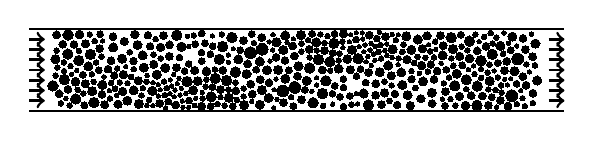
\begin{tikzpicture}[
scale=2.0,
]

\foreach \y in {0.65,1.3,1.95,2.6,3.25,3.9,4.55}
  \draw[color=black,line width=1.0pt,solid,->]
      (0mm,\y mm) -- (1mm, \y mm);
% inlet arrow

\foreach \y in {0.65,1.3,1.95,2.6,3.25,3.9,4.55}
  \draw[color=black,line width=1.0pt,solid,->]
      (33mm,\y mm) -- (34mm, \y mm);
% outlet arrow

% outer walls
\draw[line width=1pt] (0mm,0mm) -- (34mm,0mm);
\draw[line width=1pt] (0mm,5.2mm) -- (34mm,5.2mm);
\filldraw[line width=0pt] (31.902159mm,4.880683mm) circle (0.139755mm);
\filldraw[line width=0pt] (10.132162mm,4.093149mm) circle (0.138503mm);
\filldraw[line width=0pt] (30.969474mm,4.127407mm) circle (0.139086mm);
\filldraw[line width=0pt] (30.444063mm,4.291359mm) circle (0.138665mm);
\filldraw[line width=0pt] (30.148560mm,4.952732mm) circle (0.139398mm);
\filldraw[line width=0pt] (21.259932mm,3.757617mm) circle (0.138874mm);
\filldraw[line width=0pt] (4.676123mm,4.447397mm) circle (0.138741mm);
\filldraw[line width=0pt] (8.949880mm,1.101227mm) circle (0.137175mm);
\filldraw[line width=0pt] (22.592900mm,3.845908mm) circle (0.137855mm);
\filldraw[line width=0pt] (8.674888mm,0.201377mm) circle (0.139054mm);
\filldraw[line width=0pt] (14.143777mm,0.611821mm) circle (0.139339mm);
\filldraw[line width=0pt] (31.224078mm,1.289528mm) circle (0.138869mm);
\filldraw[line width=0pt] (15.487198mm,4.844206mm) circle (0.139782mm);
\filldraw[line width=0pt] (31.771043mm,2.480915mm) circle (0.139632mm);
\filldraw[line width=0pt] (9.407770mm,1.736749mm) circle (0.138835mm);
\filldraw[line width=0pt] (9.770237mm,0.236518mm) circle (0.138513mm);
\filldraw[line width=0pt] (15.291087mm,3.166535mm) circle (0.139854mm);
\filldraw[line width=0pt] (9.963742mm,1.109633mm) circle (0.139531mm);
\filldraw[line width=0pt] (20.792104mm,1.103777mm) circle (0.138848mm);
\filldraw[line width=0pt] (24.789923mm,2.381274mm) circle (0.139043mm);
\filldraw[line width=0pt] (22.249380mm,4.994797mm) circle (0.139155mm);
\filldraw[line width=0pt] (27.901102mm,2.626849mm) circle (0.139921mm);
\filldraw[line width=0pt] (16.384172mm,4.348901mm) circle (0.138589mm);
\filldraw[line width=0pt] (19.927414mm,4.014550mm) circle (0.139057mm);
\filldraw[line width=0pt] (6.133579mm,2.816454mm) circle (0.139181mm);
\filldraw[line width=0pt] (7.864709mm,0.334403mm) circle (0.139534mm);
\filldraw[line width=0pt] (15.746136mm,0.743515mm) circle (0.139109mm);
\filldraw[line width=0pt] (7.872138mm,1.797924mm) circle (0.138905mm);
\filldraw[line width=0pt] (15.540087mm,0.202128mm) circle (0.139979mm);
\filldraw[line width=0pt] (10.503964mm,0.348933mm) circle (0.139480mm);
\filldraw[line width=0pt] (9.665134mm,1.437424mm) circle (0.138971mm);
\filldraw[line width=0pt] (8.964672mm,1.975267mm) circle (0.138265mm);
\filldraw[line width=0pt] (10.063356mm,4.741980mm) circle (0.139579mm);
\filldraw[line width=0pt] (23.428188mm,2.945236mm) circle (0.139033mm);
\filldraw[line width=0pt] (21.650636mm,3.870711mm) circle (0.138217mm);
\filldraw[line width=0pt] (30.376882mm,1.649633mm) circle (0.138764mm);
\filldraw[line width=0pt] (9.729186mm,0.625280mm) circle (0.137022mm);
\filldraw[line width=0pt] (23.061298mm,4.861263mm) circle (0.138821mm);
\filldraw[line width=0pt] (20.863424mm,0.454159mm) circle (0.140199mm);
\filldraw[line width=0pt] (20.958077mm,4.087251mm) circle (0.137443mm);
\filldraw[line width=0pt] (9.055093mm,1.585056mm) circle (0.138885mm);
\filldraw[line width=0pt] (11.641671mm,4.764299mm) circle (0.139807mm);
\filldraw[line width=0pt] (22.717519mm,3.520873mm) circle (0.139085mm);
\filldraw[line width=0pt] (8.332031mm,1.349266mm) circle (0.138229mm);
\filldraw[line width=0pt] (18.267159mm,1.643874mm) circle (0.139483mm);
\filldraw[line width=0pt] (20.420929mm,4.845512mm) circle (0.138853mm);
\filldraw[line width=0pt] (19.282100mm,0.429216mm) circle (0.139476mm);
\filldraw[line width=0pt] (21.189264mm,4.569077mm) circle (0.137595mm);
\filldraw[line width=0pt] (28.225031mm,2.864593mm) circle (0.139409mm);
\filldraw[line width=0pt] (12.660696mm,3.086504mm) circle (0.139114mm);
\filldraw[line width=0pt] (3.027663mm,2.565862mm) circle (0.139737mm);
\filldraw[line width=0pt] (15.245500mm,4.387543mm) circle (0.139551mm);
\filldraw[line width=0pt] (21.868004mm,3.608024mm) circle (0.138429mm);
\filldraw[line width=0pt] (12.967269mm,3.946799mm) circle (0.139354mm);
\filldraw[line width=0pt] (30.201523mm,2.010995mm) circle (0.138334mm);
\filldraw[line width=0pt] (25.824675mm,3.900396mm) circle (0.139460mm);
\filldraw[line width=0pt] (9.274736mm,1.321411mm) circle (0.138983mm);
\filldraw[line width=0pt] (21.957960mm,3.218185mm) circle (0.138919mm);
\filldraw[line width=0pt] (21.975109mm,4.092289mm) circle (0.138324mm);
\filldraw[line width=0pt] (12.655784mm,3.551719mm) circle (0.137841mm);
\filldraw[line width=0pt] (10.995816mm,1.179620mm) circle (0.139468mm);
\filldraw[line width=0pt] (26.167414mm,3.030902mm) circle (0.139579mm);
\filldraw[line width=0pt] (23.054766mm,3.394457mm) circle (0.139667mm);
\filldraw[line width=0pt] (10.581130mm,0.800518mm) circle (0.139182mm);
\filldraw[line width=0pt] (21.341521mm,4.190331mm) circle (0.138807mm);
\filldraw[line width=0pt] (30.583859mm,2.050804mm) circle (0.138201mm);
\filldraw[line width=0pt] (26.247310mm,0.751561mm) circle (0.139028mm);
\filldraw[line width=0pt] (2.698244mm,2.327257mm) circle (0.138968mm);
\filldraw[line width=0pt] (29.688680mm,0.242872mm) circle (0.139191mm);
\filldraw[line width=0pt] (20.781365mm,4.968799mm) circle (0.137309mm);
\filldraw[line width=0pt] (16.782393mm,4.582307mm) circle (0.138570mm);
\filldraw[line width=0pt] (28.580833mm,4.403333mm) circle (0.138888mm);
\filldraw[line width=0pt] (21.515240mm,3.456316mm) circle (0.137601mm);
\filldraw[line width=0pt] (4.757410mm,2.168123mm) circle (0.140106mm);
\filldraw[line width=0pt] (9.214564mm,0.901229mm) circle (0.139110mm);
\filldraw[line width=0pt] (7.496260mm,2.251082mm) circle (0.139057mm);
\filldraw[line width=0pt] (18.261335mm,2.110241mm) circle (0.139110mm);
\filldraw[line width=0pt] (20.341497mm,4.393136mm) circle (0.138507mm);
\filldraw[line width=0pt] (7.481159mm,0.351066mm) circle (0.138118mm);
\filldraw[line width=0pt] (9.520040mm,2.074033mm) circle (0.139255mm);
\filldraw[line width=0pt] (23.439970mm,4.841358mm) circle (0.137661mm);
\filldraw[line width=0pt] (5.101877mm,1.294747mm) circle (0.139523mm);
\filldraw[line width=0pt] (21.735784mm,2.883067mm) circle (0.139225mm);
\filldraw[line width=0pt] (22.716201mm,4.253426mm) circle (0.138348mm);
\filldraw[line width=0pt] (29.534671mm,2.545359mm) circle (0.138982mm);
\filldraw[line width=0pt] (21.400171mm,3.123176mm) circle (0.138900mm);
\filldraw[line width=0pt] (15.559736mm,1.344829mm) circle (0.138163mm);
\filldraw[line width=0pt] (9.186667mm,2.311044mm) circle (0.139755mm);
\filldraw[line width=0pt] (9.585112mm,1.004652mm) circle (0.137857mm);
\filldraw[line width=0pt] (21.154137mm,4.960067mm) circle (0.138783mm);
\filldraw[line width=0pt] (15.681852mm,2.019302mm) circle (0.139392mm);
\filldraw[line width=0pt] (21.710525mm,4.296754mm) circle (0.139008mm);
\filldraw[line width=0pt] (15.470186mm,3.872658mm) circle (0.139940mm);
\filldraw[line width=0pt] (5.557064mm,0.984788mm) circle (0.138570mm);
\filldraw[line width=0pt] (2.340986mm,0.794282mm) circle (0.138672mm);
\filldraw[line width=0pt] (10.137902mm,0.228416mm) circle (0.138015mm);
\filldraw[line width=0pt] (17.956522mm,1.247480mm) circle (0.138220mm);
\filldraw[line width=0pt] (8.205326mm,0.943781mm) circle (0.139195mm);
\filldraw[line width=0pt] (8.206317mm,1.673469mm) circle (0.138562mm);
\filldraw[line width=0pt] (22.889491mm,0.637058mm) circle (0.175587mm);
\filldraw[line width=0pt] (23.018951mm,1.621364mm) circle (0.174911mm);
\filldraw[line width=0pt] (24.669577mm,3.432819mm) circle (0.174082mm);
\filldraw[line width=0pt] (4.254197mm,3.068418mm) circle (0.175321mm);
\filldraw[line width=0pt] (23.783605mm,4.209925mm) circle (0.175543mm);
\filldraw[line width=0pt] (29.316573mm,4.947144mm) circle (0.175421mm);
\filldraw[line width=0pt] (10.460252mm,4.801014mm) circle (0.175148mm);
\filldraw[line width=0pt] (26.667557mm,2.126338mm) circle (0.174294mm);
\filldraw[line width=0pt] (18.766931mm,4.317711mm) circle (0.173527mm);
\filldraw[line width=0pt] (22.307918mm,4.189890mm) circle (0.174642mm);
\filldraw[line width=0pt] (19.666447mm,3.210020mm) circle (0.174702mm);
\filldraw[line width=0pt] (20.465058mm,0.393284mm) circle (0.175076mm);
\filldraw[line width=0pt] (27.761746mm,1.379426mm) circle (0.176149mm);
\filldraw[line width=0pt] (13.631287mm,1.423917mm) circle (0.174417mm);
\filldraw[line width=0pt] (13.617280mm,0.921188mm) circle (0.173592mm);
\filldraw[line width=0pt] (3.989987mm,2.328826mm) circle (0.174538mm);
\filldraw[line width=0pt] (31.336718mm,0.809517mm) circle (0.174677mm);
\filldraw[line width=0pt] (2.221851mm,2.538811mm) circle (0.173186mm);
\filldraw[line width=0pt] (5.598661mm,2.704560mm) circle (0.175394mm);
\filldraw[line width=0pt] (28.712823mm,2.104499mm) circle (0.174247mm);
\filldraw[line width=0pt] (29.667097mm,4.660586mm) circle (0.175887mm);
\filldraw[line width=0pt] (12.158850mm,0.878742mm) circle (0.174327mm);
\filldraw[line width=0pt] (29.238444mm,2.945010mm) circle (0.175240mm);
\filldraw[line width=0pt] (6.254025mm,1.763206mm) circle (0.175109mm);
\filldraw[line width=0pt] (26.935087mm,2.869958mm) circle (0.176220mm);
\filldraw[line width=0pt] (14.280337mm,4.315607mm) circle (0.175268mm);
\filldraw[line width=0pt] (3.859922mm,4.856019mm) circle (0.174911mm);
\filldraw[line width=0pt] (4.167217mm,4.438767mm) circle (0.174911mm);
\filldraw[line width=0pt] (29.768694mm,2.135064mm) circle (0.174997mm);
\filldraw[line width=0pt] (12.246212mm,4.865084mm) circle (0.175500mm);
\filldraw[line width=0pt] (28.699509mm,2.654005mm) circle (0.173187mm);
\filldraw[line width=0pt] (29.442422mm,4.282195mm) circle (0.173920mm);
\filldraw[line width=0pt] (7.139541mm,0.985667mm) circle (0.174881mm);
\filldraw[line width=0pt] (30.978341mm,0.429468mm) circle (0.174816mm);
\filldraw[line width=0pt] (26.816909mm,3.344743mm) circle (0.175674mm);
\filldraw[line width=0pt] (28.288581mm,2.344131mm) circle (0.174908mm);
\filldraw[line width=0pt] (17.727532mm,4.490595mm) circle (0.174553mm);
\filldraw[line width=0pt] (28.338436mm,4.852768mm) circle (0.174017mm);
\filldraw[line width=0pt] (25.368926mm,4.210926mm) circle (0.139087mm);
\filldraw[line width=0pt] (29.124408mm,2.435447mm) circle (0.174604mm);
\filldraw[line width=0pt] (17.306441mm,4.269562mm) circle (0.174273mm);
\filldraw[line width=0pt] (17.294135mm,3.773496mm) circle (0.174779mm);
\filldraw[line width=0pt] (2.583863mm,0.342728mm) circle (0.175112mm);
\filldraw[line width=0pt] (31.482526mm,0.305858mm) circle (0.174744mm);
\filldraw[line width=0pt] (19.120074mm,2.561459mm) circle (0.173902mm);
\filldraw[line width=0pt] (17.814921mm,3.395546mm) circle (0.175662mm);
\filldraw[line width=0pt] (2.635886mm,2.849353mm) circle (0.175431mm);
\filldraw[line width=0pt] (5.761396mm,1.813773mm) circle (0.173855mm);
\filldraw[line width=0pt] (1.758605mm,3.823196mm) circle (0.175100mm);
\filldraw[line width=0pt] (18.956710mm,4.754144mm) circle (0.174849mm);
\filldraw[line width=0pt] (23.293093mm,4.492919mm) circle (0.175808mm);
\filldraw[line width=0pt] (25.163686mm,3.377039mm) circle (0.174465mm);
\filldraw[line width=0pt] (11.208832mm,1.550597mm) circle (0.173996mm);
\filldraw[line width=0pt] (1.799736mm,2.760888mm) circle (0.175265mm);
\filldraw[line width=0pt] (26.333912mm,1.757959mm) circle (0.175562mm);
\filldraw[line width=0pt] (2.022174mm,0.485836mm) circle (0.175011mm);
\filldraw[line width=0pt] (1.687421mm,2.249053mm) circle (0.175240mm);
\filldraw[line width=0pt] (30.100719mm,3.633031mm) circle (0.175650mm);
\filldraw[line width=0pt] (29.972827mm,1.628562mm) circle (0.174794mm);
\filldraw[line width=0pt] (3.157987mm,3.814339mm) circle (0.174742mm);
\filldraw[line width=0pt] (27.835200mm,3.851379mm) circle (0.175358mm);
\filldraw[line width=0pt] (22.351742mm,3.323650mm) circle (0.172390mm);
\filldraw[line width=0pt] (26.759592mm,0.758441mm) circle (0.174609mm);
\filldraw[line width=0pt] (23.699647mm,3.749544mm) circle (0.175656mm);
\filldraw[line width=0pt] (13.109305mm,1.800490mm) circle (0.176010mm);
\filldraw[line width=0pt] (28.899223mm,4.706869mm) circle (0.173675mm);
\filldraw[line width=0pt] (23.465632mm,3.341794mm) circle (0.174759mm);
\filldraw[line width=0pt] (13.197949mm,0.708236mm) circle (0.175170mm);
\filldraw[line width=0pt] (29.612820mm,1.331179mm) circle (0.175106mm);
\filldraw[line width=0pt] (25.713998mm,3.409409mm) circle (0.175029mm);
\filldraw[line width=0pt] (6.392401mm,3.729278mm) circle (0.182493mm);
\filldraw[line width=0pt] (5.210615mm,1.787221mm) circle (0.174404mm);
\filldraw[line width=0pt] (5.139389mm,0.796689mm) circle (0.175307mm);
\filldraw[line width=0pt] (24.530531mm,1.463376mm) circle (0.182103mm);
\filldraw[line width=0pt] (6.647252mm,2.660703mm) circle (0.174795mm);
\filldraw[line width=0pt] (7.905157mm,3.571419mm) circle (0.174554mm);
\filldraw[line width=0pt] (24.276618mm,2.533909mm) circle (0.174887mm);
\filldraw[line width=0pt] (18.275326mm,3.841862mm) circle (0.173331mm);
\filldraw[line width=0pt] (24.448319mm,3.042224mm) circle (0.183092mm);
\filldraw[line width=0pt] (31.993264mm,0.496317mm) circle (0.182068mm);
\filldraw[line width=0pt] (3.450614mm,1.110648mm) circle (0.175502mm);
\filldraw[line width=0pt] (31.584697mm,2.961299mm) circle (0.174944mm);
\filldraw[line width=0pt] (27.061443mm,0.340269mm) circle (0.176070mm);
\filldraw[line width=0pt] (22.182286mm,3.746330mm) circle (0.175533mm);
\filldraw[line width=0pt] (4.106395mm,1.850536mm) circle (0.175240mm);
\filldraw[line width=0pt] (32.123961mm,2.896973mm) circle (0.182033mm);
\filldraw[line width=0pt] (12.421098mm,0.333525mm) circle (0.174669mm);
\filldraw[line width=0pt] (18.501632mm,4.863275mm) circle (0.174116mm);
\filldraw[line width=0pt] (16.645866mm,0.879041mm) circle (0.176304mm);
\filldraw[line width=0pt] (5.458788mm,1.402116mm) circle (0.182840mm);
\filldraw[line width=0pt] (11.258305mm,1.989449mm) circle (0.174337mm);
\filldraw[line width=0pt] (6.477299mm,2.157066mm) circle (0.183358mm);
\filldraw[line width=0pt] (12.649395mm,1.353810mm) circle (0.175026mm);
\filldraw[line width=0pt] (8.613054mm,1.004890mm) circle (0.175778mm);
\filldraw[line width=0pt] (18.673852mm,0.327310mm) circle (0.176480mm);
\filldraw[line width=0pt] (30.009169mm,1.160477mm) circle (0.173969mm);
\filldraw[line width=0pt] (7.630014mm,0.701137mm) circle (0.175323mm);
\filldraw[line width=0pt] (29.161950mm,1.371632mm) circle (0.173996mm);
\filldraw[line width=0pt] (8.035363mm,4.561948mm) circle (0.176237mm);
\filldraw[line width=0pt] (25.466409mm,3.794563mm) circle (0.181481mm);
\filldraw[line width=0pt] (11.800508mm,2.635709mm) circle (0.174806mm);
\filldraw[line width=0pt] (11.964952mm,0.443212mm) circle (0.175853mm);
\filldraw[line width=0pt] (7.224775mm,1.447369mm) circle (0.176442mm);
\filldraw[line width=0pt] (25.784834mm,4.400780mm) circle (0.175985mm);
\filldraw[line width=0pt] (25.327849mm,2.495087mm) circle (0.175663mm);
\filldraw[line width=0pt] (7.458653mm,1.849351mm) circle (0.175047mm);
\filldraw[line width=0pt] (11.024815mm,0.791497mm) circle (0.173501mm);
\filldraw[line width=0pt] (27.473379mm,4.086252mm) circle (0.175169mm);
\filldraw[line width=0pt] (3.092924mm,1.344155mm) circle (0.176095mm);
\filldraw[line width=0pt] (19.896484mm,4.405340mm) circle (0.173691mm);
\filldraw[line width=0pt] (2.213668mm,3.089311mm) circle (0.174785mm);
\filldraw[line width=0pt] (22.560492mm,1.860729mm) circle (0.182268mm);
\filldraw[line width=0pt] (19.711003mm,3.644348mm) circle (0.174131mm);
\filldraw[line width=0pt] (19.961547mm,2.031603mm) circle (0.214231mm);
\filldraw[line width=0pt] (8.362102mm,3.337220mm) circle (0.183979mm);
\filldraw[line width=0pt] (8.738781mm,1.447642mm) circle (0.175741mm);
\filldraw[line width=0pt] (8.570044mm,1.870747mm) circle (0.173582mm);
\filldraw[line width=0pt] (21.048364mm,2.655497mm) circle (0.215597mm);
\filldraw[line width=0pt] (11.651572mm,1.515461mm) circle (0.217859mm);
\filldraw[line width=0pt] (19.973444mm,1.488821mm) circle (0.214819mm);
\filldraw[line width=0pt] (4.589712mm,3.442332mm) circle (0.176714mm);
\filldraw[line width=0pt] (19.398615mm,4.898068mm) circle (0.218095mm);
\filldraw[line width=0pt] (11.170973mm,4.297055mm) circle (0.213169mm);
\filldraw[line width=0pt] (26.497872mm,2.616318mm) circle (0.214002mm);
\filldraw[line width=0pt] (27.414554mm,4.840253mm) circle (0.216563mm);
\filldraw[line width=0pt] (30.581854mm,3.857443mm) circle (0.217006mm);
\filldraw[line width=0pt] (27.508392mm,2.893516mm) circle (0.217371mm);
\filldraw[line width=0pt] (20.371213mm,0.952242mm) circle (0.214771mm);
\filldraw[line width=0pt] (12.942633mm,0.297053mm) circle (0.216938mm);
\filldraw[line width=0pt] (14.425632mm,2.622341mm) circle (0.218642mm);
\filldraw[line width=0pt] (16.497239mm,2.574849mm) circle (0.218593mm);
\filldraw[line width=0pt] (10.961885mm,4.923457mm) circle (0.216125mm);
\filldraw[line width=0pt] (19.264803mm,1.091921mm) circle (0.214337mm);
\filldraw[line width=0pt] (10.158045mm,0.662207mm) circle (0.214146mm);
\filldraw[line width=0pt] (10.951115mm,3.707225mm) circle (0.214433mm);
\filldraw[line width=0pt] (11.515919mm,3.598018mm) circle (0.213838mm);
\filldraw[line width=0pt] (4.512105mm,4.868637mm) circle (0.215597mm);
\filldraw[line width=0pt] (3.511021mm,0.353735mm) circle (0.217768mm);
\filldraw[line width=0pt] (10.552164mm,4.242337mm) circle (0.214840mm);
\filldraw[line width=0pt] (29.758107mm,3.050058mm) circle (0.217485mm);
\filldraw[line width=0pt] (3.416355mm,2.300814mm) circle (0.217462mm);
\filldraw[line width=0pt] (17.515155mm,1.342599mm) circle (0.217972mm);
\filldraw[line width=0pt] (19.405118mm,1.598251mm) circle (0.213835mm);
\filldraw[line width=0pt] (30.955471mm,1.724310mm) circle (0.217981mm);
\filldraw[line width=0pt] (10.962214mm,3.163724mm) circle (0.215381mm);
\filldraw[line width=0pt] (19.751576mm,0.898198mm) circle (0.212912mm);
\filldraw[line width=0pt] (10.133518mm,2.991283mm) circle (0.212927mm);
\filldraw[line width=0pt] (20.791613mm,2.205220mm) circle (0.213204mm);
\filldraw[line width=0pt] (9.877854mm,2.542461mm) circle (0.213577mm);
\filldraw[line width=0pt] (26.412947mm,0.329289mm) circle (0.214186mm);
\filldraw[line width=0pt] (21.373565mm,1.798386mm) circle (0.214017mm);
\filldraw[line width=0pt] (11.657232mm,4.105820mm) circle (0.212476mm);
\filldraw[line width=0pt] (4.425596mm,2.581928mm) circle (0.213470mm);
\filldraw[line width=0pt] (29.386590mm,0.878674mm) circle (0.217522mm);
\filldraw[line width=0pt] (9.548803mm,3.395039mm) circle (0.214759mm);
\filldraw[line width=0pt] (19.962446mm,0.272399mm) circle (0.214251mm);
\filldraw[line width=0pt] (8.842779mm,0.594422mm) circle (0.215726mm);
\filldraw[line width=0pt] (22.080896mm,4.599083mm) circle (0.216104mm);
\filldraw[line width=0pt] (11.528839mm,0.299972mm) circle (0.218532mm);
\filldraw[line width=0pt] (13.407378mm,3.852066mm) circle (0.216709mm);
\filldraw[line width=0pt] (31.979358mm,3.442380mm) circle (0.246966mm);
\filldraw[line width=0pt] (16.787215mm,0.310727mm) circle (0.219276mm);
\filldraw[line width=0pt] (20.766088mm,4.534097mm) circle (0.213321mm);
\filldraw[line width=0pt] (29.926432mm,0.675381mm) circle (0.246902mm);
\filldraw[line width=0pt] (30.413971mm,0.316716mm) circle (0.246811mm);
\filldraw[line width=0pt] (17.982835mm,4.898130mm) circle (0.216144mm);
\filldraw[line width=0pt] (5.330605mm,4.721111mm) circle (0.246989mm);
\filldraw[line width=0pt] (14.138609mm,4.881951mm) circle (0.217231mm);
\filldraw[line width=0pt] (26.119223mm,4.794916mm) circle (0.246684mm);
\filldraw[line width=0pt] (28.782958mm,0.954496mm) circle (0.246457mm);
\filldraw[line width=0pt] (2.850270mm,4.220288mm) circle (0.247355mm);
\filldraw[line width=0pt] (31.356957mm,2.184128mm) circle (0.246757mm);
\filldraw[line width=0pt] (1.755281mm,4.833714mm) circle (0.246717mm);
\filldraw[line width=0pt] (13.880037mm,2.988786mm) circle (0.246768mm);
\filldraw[line width=0pt] (14.678531mm,1.990034mm) circle (0.247083mm);
\filldraw[line width=0pt] (23.378238mm,0.385170mm) circle (0.234931mm);
\filldraw[line width=0pt] (5.014255mm,2.658447mm) circle (0.246110mm);
\filldraw[line width=0pt] (24.292345mm,2.024951mm) circle (0.234784mm);
\filldraw[line width=0pt] (23.232451mm,1.085502mm) circle (0.234988mm);
\filldraw[line width=0pt] (15.238218mm,1.790124mm) circle (0.247384mm);
\filldraw[line width=0pt] (25.510362mm,2.945147mm) circle (0.234910mm);
\filldraw[line width=0pt] (19.274463mm,3.681464mm) circle (0.217412mm);
\filldraw[line width=0pt] (22.388903mm,0.401819mm) circle (0.246625mm);
\filldraw[line width=0pt] (17.799368mm,3.916697mm) circle (0.247408mm);
\filldraw[line width=0pt] (28.454802mm,3.820798mm) circle (0.246563mm);
\filldraw[line width=0pt] (16.747954mm,4.127669mm) circle (0.246810mm);
\filldraw[line width=0pt] (7.544650mm,4.810411mm) circle (0.234781mm);
\filldraw[line width=0pt] (26.438053mm,1.229725mm) circle (0.247019mm);
\filldraw[line width=0pt] (31.363568mm,4.602637mm) circle (0.246832mm);
\filldraw[line width=0pt] (30.333856mm,3.149317mm) circle (0.247936mm);
\filldraw[line width=0pt] (25.594005mm,0.473317mm) circle (0.247330mm);
\filldraw[line width=0pt] (8.922352mm,4.196783mm) circle (0.247330mm);
\filldraw[line width=0pt] (14.778004mm,4.667525mm) circle (0.247045mm);
\filldraw[line width=0pt] (4.485629mm,3.964793mm) circle (0.247400mm);
\filldraw[line width=0pt] (16.245979mm,3.205085mm) circle (0.246870mm);
\filldraw[line width=0pt] (25.910213mm,2.535864mm) circle (0.247051mm);
\filldraw[line width=0pt] (6.042267mm,4.416632mm) circle (0.259461mm);
\filldraw[line width=0pt] (9.316687mm,0.380225mm) circle (0.246524mm);
\filldraw[line width=0pt] (5.208660mm,3.188712mm) circle (0.248072mm);
\filldraw[line width=0pt] (18.620745mm,2.606416mm) circle (0.246998mm);
\filldraw[line width=0pt] (5.412980mm,2.248860mm) circle (0.233972mm);
\filldraw[line width=0pt] (29.167968mm,0.359570mm) circle (0.247211mm);
\filldraw[line width=0pt] (21.603878mm,4.811253mm) circle (0.247636mm);
\filldraw[line width=0pt] (8.535077mm,4.794019mm) circle (0.247332mm);
\filldraw[line width=0pt] (8.906492mm,3.467749mm) circle (0.247034mm);
\filldraw[line width=0pt] (16.849883mm,3.496118mm) circle (0.246448mm);
\filldraw[line width=0pt] (31.996306mm,1.129844mm) circle (0.247125mm);
\filldraw[line width=0pt] (25.716075mm,2.004908mm) circle (0.247123mm);
\filldraw[line width=0pt] (4.628403mm,1.054834mm) circle (0.246401mm);
\filldraw[line width=0pt] (3.587249mm,4.261905mm) circle (0.259221mm);
\filldraw[line width=0pt] (28.073239mm,0.977061mm) circle (0.246873mm);
\filldraw[line width=0pt] (17.046463mm,2.209544mm) circle (0.246873mm);
\filldraw[line width=0pt] (7.688161mm,4.109231mm) circle (0.235072mm);
\filldraw[line width=0pt] (24.883945mm,0.778378mm) circle (0.259786mm);
\filldraw[line width=0pt] (22.632004mm,4.714140mm) circle (0.246891mm);
\filldraw[line width=0pt] (27.334294mm,0.933972mm) circle (0.259797mm);
\filldraw[line width=0pt] (30.185274mm,2.562040mm) circle (0.247791mm);
\filldraw[line width=0pt] (18.765930mm,3.828768mm) circle (0.247546mm);
\filldraw[line width=0pt] (6.626389mm,3.169561mm) circle (0.235431mm);
\filldraw[line width=0pt] (8.295639mm,0.481049mm) circle (0.247632mm);
\filldraw[line width=0pt] (2.468101mm,1.377149mm) circle (0.246803mm);
\filldraw[line width=0pt] (13.124906mm,1.281216mm) circle (0.246543mm);
\filldraw[line width=0pt] (7.924591mm,2.961275mm) circle (0.259222mm);
\filldraw[line width=0pt] (22.004487mm,1.000612mm) circle (0.247709mm);
\filldraw[line width=0pt] (31.510330mm,3.902079mm) circle (0.247443mm);
\filldraw[line width=0pt] (9.357122mm,2.747806mm) circle (0.247348mm);
\filldraw[line width=0pt] (2.142291mm,4.238869mm) circle (0.246433mm);
\filldraw[line width=0pt] (1.911025mm,1.089591mm) circle (0.247449mm);
\filldraw[line width=0pt] (15.685116mm,3.406057mm) circle (0.247617mm);
\filldraw[line width=0pt] (14.174729mm,1.067502mm) circle (0.246460mm);
\filldraw[line width=0pt] (6.716867mm,4.856612mm) circle (0.266196mm);
\filldraw[line width=0pt] (12.158461mm,1.366622mm) circle (0.246830mm);
\filldraw[line width=0pt] (19.966646mm,4.897554mm) circle (0.260389mm);
\filldraw[line width=0pt] (29.014059mm,4.106865mm) circle (0.247027mm);
\filldraw[line width=0pt] (14.073728mm,1.703404mm) circle (0.248930mm);
\filldraw[line width=0pt] (6.927002mm,1.921610mm) circle (0.260327mm);
\filldraw[line width=0pt] (13.617877mm,4.483907mm) circle (0.246717mm);
\filldraw[line width=0pt] (23.000560mm,2.234343mm) circle (0.260333mm);
\filldraw[line width=0pt] (25.270989mm,4.768221mm) circle (0.260414mm);
\filldraw[line width=0pt] (24.207682mm,0.338252mm) circle (0.266188mm);
\filldraw[line width=0pt] (5.652679mm,0.427657mm) circle (0.259552mm);
\filldraw[line width=0pt] (12.302011mm,2.586686mm) circle (0.247073mm);
\filldraw[line width=0pt] (27.352330mm,3.467596mm) circle (0.260438mm);
\filldraw[line width=0pt] (5.951667mm,1.238074mm) circle (0.266840mm);
\filldraw[line width=0pt] (3.570883mm,1.728318mm) circle (0.260248mm);
\filldraw[line width=0pt] (20.403439mm,2.619050mm) circle (0.260660mm);
\filldraw[line width=0pt] (31.555874mm,1.637019mm) circle (0.247329mm);
\filldraw[line width=0pt] (24.976013mm,3.956404mm) circle (0.266681mm);
\filldraw[line width=0pt] (10.956286mm,0.296757mm) circle (0.260332mm);
\filldraw[line width=0pt] (22.571286mm,1.149903mm) circle (0.266181mm);
\filldraw[line width=0pt] (23.999240mm,3.274000mm) circle (0.260128mm);
\filldraw[line width=0pt] (8.352453mm,4.046981mm) circle (0.265668mm);
\filldraw[line width=0pt] (21.564880mm,2.447521mm) circle (0.249152mm);
\filldraw[line width=0pt] (24.037528mm,1.007271mm) circle (0.285796mm);
\filldraw[line width=0pt] (14.650236mm,3.141452mm) circle (0.289018mm);
\filldraw[line width=0pt] (17.303424mm,0.711623mm) circle (0.247856mm);
\filldraw[line width=0pt] (4.804021mm,0.401093mm) circle (0.248961mm);
\filldraw[line width=0pt] (26.297828mm,4.143328mm) circle (0.248654mm);
\filldraw[line width=0pt] (10.519229mm,2.574028mm) circle (0.260364mm);
\filldraw[line width=0pt] (10.718068mm,1.900168mm) circle (0.278923mm);
\filldraw[line width=0pt] (22.018465mm,1.730159mm) circle (0.247170mm);
\filldraw[line width=0pt] (2.948445mm,1.860154mm) circle (0.279278mm);
\filldraw[line width=0pt] (24.927755mm,2.885253mm) circle (0.265980mm);
\filldraw[line width=0pt] (16.148622mm,0.528168mm) circle (0.247149mm);
\filldraw[line width=0pt] (30.694065mm,4.719179mm) circle (0.287640mm);
\filldraw[line width=0pt] (5.992685mm,2.308650mm) circle (0.266257mm);
\filldraw[line width=0pt] (6.886977mm,4.190822mm) circle (0.285872mm);
\filldraw[line width=0pt] (15.815287mm,2.610195mm) circle (0.287863mm);
\filldraw[line width=0pt] (15.109778mm,2.585805mm) circle (0.287703mm);
\filldraw[line width=0pt] (6.644128mm,1.313357mm) circle (0.285879mm);
\filldraw[line width=0pt] (11.262098mm,2.512880mm) circle (0.279099mm);
\filldraw[line width=0pt] (30.823246mm,2.528012mm) circle (0.288220mm);
\filldraw[line width=0pt] (17.634108mm,1.914813mm) circle (0.287666mm);
\filldraw[line width=0pt] (7.215603mm,3.535801mm) circle (0.285337mm);
\filldraw[line width=0pt] (32.264181mm,1.936298mm) circle (0.288835mm);
\filldraw[line width=0pt] (16.277951mm,2.051619mm) circle (0.288059mm);
\filldraw[line width=0pt] (20.207204mm,3.297794mm) circle (0.279684mm);
\filldraw[line width=0pt] (16.144202mm,3.870733mm) circle (0.288787mm);
\filldraw[line width=0pt] (13.812802mm,2.346938mm) circle (0.287863mm);
\filldraw[line width=0pt] (5.346621mm,4.035213mm) circle (0.289110mm);
\filldraw[line width=0pt] (21.244020mm,1.113139mm) circle (0.291096mm);
\filldraw[line width=0pt] (15.212352mm,0.829550mm) circle (0.287856mm);
\filldraw[line width=0pt] (29.930266mm,4.132884mm) circle (0.289975mm);
\filldraw[line width=0pt] (25.018296mm,1.876399mm) circle (0.288720mm);
\filldraw[line width=0pt] (8.651224mm,2.735777mm) circle (0.288496mm);
\filldraw[line width=0pt] (23.637639mm,2.443873mm) circle (0.285130mm);
\filldraw[line width=0pt] (14.783037mm,1.325871mm) circle (0.288183mm);
\filldraw[line width=0pt] (17.109957mm,2.847011mm) circle (0.287945mm);
\filldraw[line width=0pt] (6.970174mm,0.450130mm) circle (0.290425mm);
\filldraw[line width=0pt] (27.720608mm,0.345050mm) circle (0.279325mm);
\filldraw[line width=0pt] (14.656618mm,0.397870mm) circle (0.285269mm);
\filldraw[line width=0pt] (20.509286mm,3.883179mm) circle (0.290195mm);
\filldraw[line width=0pt] (5.908782mm,3.319853mm) circle (0.288671mm);
\filldraw[line width=0pt] (4.009092mm,1.255762mm) circle (0.290035mm);
\filldraw[line width=0pt] (19.659370mm,2.682576mm) circle (0.280405mm);
\filldraw[line width=0pt] (7.287332mm,2.755798mm) circle (0.286333mm);
\filldraw[line width=0pt] (26.913452mm,3.939239mm) circle (0.289258mm);
\filldraw[line width=0pt] (23.952617mm,4.747323mm) circle (0.289828mm);
\filldraw[line width=0pt] (23.092122mm,3.922701mm) circle (0.290399mm);
\filldraw[line width=0pt] (13.291079mm,3.279358mm) circle (0.289388mm);
\filldraw[line width=0pt] (7.831719mm,1.275177mm) circle (0.294774mm);
\filldraw[line width=0pt] (25.578431mm,1.158469mm) circle (0.290137mm);
\filldraw[line width=0pt] (24.279369mm,3.886159mm) circle (0.285807mm);
\filldraw[line width=0pt] (23.707936mm,1.656794mm) circle (0.285075mm);
\filldraw[line width=0pt] (32.156106mm,4.279946mm) circle (0.288596mm);
\filldraw[line width=0pt] (4.658632mm,1.659609mm) circle (0.289217mm);
\filldraw[line width=0pt] (27.974273mm,3.333543mm) circle (0.279208mm);
\filldraw[line width=0pt] (15.709568mm,4.361499mm) circle (0.293098mm);
\filldraw[line width=0pt] (8.115328mm,2.308957mm) circle (0.289376mm);
\filldraw[line width=0pt] (27.153079mm,2.366007mm) circle (0.289835mm);
\filldraw[line width=0pt] (6.244382mm,0.655568mm) circle (0.288198mm);
\filldraw[line width=0pt] (9.680667mm,4.084281mm) circle (0.292300mm);
\filldraw[line width=0pt] (22.269102mm,2.463210mm) circle (0.288990mm);
\filldraw[line width=0pt] (3.204252mm,4.850607mm) circle (0.279762mm);
\filldraw[line width=0pt] (22.808094mm,2.884079mm) circle (0.288912mm);
\filldraw[line width=0pt] (13.660080mm,0.378388mm) circle (0.290706mm);
\filldraw[line width=0pt] (10.415059mm,1.310876mm) circle (0.289033mm);
\filldraw[line width=0pt] (1.672317mm,3.292116mm) circle (0.290106mm);
\filldraw[line width=0pt] (24.681244mm,4.539631mm) circle (0.289049mm);
\filldraw[line width=0pt] (17.266569mm,4.814822mm) circle (0.290240mm);
\filldraw[line width=0pt] (26.264748mm,3.528486mm) circle (0.288998mm);
\filldraw[line width=0pt] (29.249521mm,1.901027mm) circle (0.290225mm);
\filldraw[line width=0pt] (3.767654mm,2.832642mm) circle (0.289974mm);
\filldraw[line width=0pt] (18.235734mm,4.358213mm) circle (0.291912mm);
\filldraw[line width=0pt] (3.158452mm,3.209124mm) circle (0.325521mm);
\filldraw[line width=0pt] (16.265575mm,4.795510mm) circle (0.287472mm);
\filldraw[line width=0pt] (12.690258mm,0.838873mm) circle (0.290913mm);
\filldraw[line width=0pt] (2.962542mm,0.761694mm) circle (0.327425mm);
\filldraw[line width=0pt] (21.546072mm,0.383547mm) circle (0.330533mm);
\filldraw[line width=0pt] (20.894580mm,3.323272mm) circle (0.332241mm);
\filldraw[line width=0pt] (2.461316mm,3.617426mm) circle (0.326281mm);
\filldraw[line width=0pt] (28.441650mm,0.361602mm) circle (0.330588mm);
\filldraw[line width=0pt] (27.031346mm,1.600566mm) circle (0.331571mm);
\filldraw[line width=0pt] (11.823175mm,2.072724mm) circle (0.326882mm);
\filldraw[line width=0pt] (13.100491mm,2.465139mm) circle (0.331293mm);
\filldraw[line width=0pt] (28.461687mm,1.577583mm) circle (0.325415mm);
\filldraw[line width=0pt] (3.894523mm,3.595722mm) circle (0.331263mm);
\filldraw[line width=0pt] (27.965447mm,4.434735mm) circle (0.327513mm);
\filldraw[line width=0pt] (12.079982mm,3.279811mm) circle (0.330977mm);
\filldraw[line width=0pt] (10.030765mm,1.870511mm) circle (0.332313mm);
\filldraw[line width=0pt] (11.565929mm,0.900394mm) circle (0.325158mm);
\filldraw[line width=0pt] (12.545474mm,1.935869mm) circle (0.332436mm);
\filldraw[line width=0pt] (19.104899mm,3.128058mm) circle (0.327429mm);
\filldraw[line width=0pt] (2.479701mm,4.830947mm) circle (0.331956mm);
\filldraw[line width=0pt] (18.037258mm,0.522011mm) circle (0.331472mm);
\filldraw[line width=0pt] (29.412730mm,3.600798mm) circle (0.331074mm);
\filldraw[line width=0pt] (4.117483mm,0.536062mm) circle (0.331269mm);
\filldraw[line width=0pt] (26.806863mm,4.660372mm) circle (0.331423mm);
\filldraw[line width=0pt] (17.818928mm,2.727494mm) circle (0.331153mm);
\filldraw[line width=0pt] (12.291910mm,4.089987mm) circle (0.331529mm);
\filldraw[line width=0pt] (27.766425mm,1.987276mm) circle (0.325038mm);
\filldraw[line width=0pt] (18.631137mm,1.106164mm) circle (0.331228mm);
\filldraw[line width=0pt] (2.235046mm,1.997505mm) circle (0.333560mm);
\filldraw[line width=0pt] (9.376923mm,4.810977mm) circle (0.331069mm);
\filldraw[line width=0pt] (1.511951mm,1.596302mm) circle (0.330901mm);
\filldraw[line width=0pt] (12.883138mm,4.671071mm) circle (0.331254mm);
\filldraw[line width=0pt] (18.843142mm,1.916167mm) circle (0.331180mm);
\filldraw[line width=0pt] (28.692751mm,3.194530mm) circle (0.333741mm);
\filldraw[line width=0pt] (18.379338mm,3.259475mm) circle (0.332865mm);
\filldraw[line width=0pt] (19.360491mm,4.296554mm) circle (0.325356mm);
\filldraw[line width=0pt] (14.058245mm,3.700290mm) circle (0.372957mm);
\filldraw[line width=0pt] (16.868633mm,1.493581mm) circle (0.372898mm);
\filldraw[line width=0pt] (16.113202mm,1.273165mm) circle (0.373588mm);
\filldraw[line width=0pt] (30.648525mm,0.970660mm) circle (0.373598mm);
\filldraw[line width=0pt] (14.807191mm,3.920906mm) circle (0.373858mm);
\filldraw[line width=0pt] (31.026645mm,3.304579mm) circle (0.373711mm);

\end{tikzpicture}

\else
  \includegraphics{circleGrains.pdf}
\fi
\caption{\label{f:beans} This geometry, which we call the {\em circle
geometry}, consists of 465 circular exclusions and has a porosity (the
ratio of the region that contains the fluid) of 0.46.  The outer wall
is denoted by $\Gamma_{0}$, and the boundary of the inner exclusions by
$\Gamma_{k}$, $k=1,\ldots,465$.}
\end{figure}


%%%%%%%%%%%%%%%%%%%%%%%%%%%%%%%%%%%%%%%%%%%%%%%%%%%%%%%%%%%%%%%%%%%%%%%%
{\em Experimental setup.}---Pietro discuses the
\begin{itemize}
  \item Experimental design
  \item Paramters and main variables
  \item Experimental methodologies
  \item PIV
\end{itemize}

%%%%%%%%%%%%%%%%%%%%%%%%%%%%%%%%%%%%%%%%%%%%%%%%%%%%%%%%%%%%%%%%%%%%%%%%
{\em Numerical solution.}---We are interested in solving Stokes
equations
\begin{align}
  \mu \Delta \uu  = \grad p, \qquad \grad \cdot \uu = 0,
  \label{e:stokes}
\end{align}
with the no-slip boundary condition $\uu = \ff$.  We use a boundary
integral equation since they naturally handle complex geometries, do
not suffer from ill-conditioning associated with direct discretizations
of~\eqref{e:stokes}, achieve high-order accuracy by using appropriate
quadrature formulae, analytically satisfy the incompressibility
condition, and can be efficiently solved iteratively by using the fast
multipole method (FMM).  Given a domain $\Omega$ with boundary
$\Gamma$, and a target point $\xx \in \Omega \backslash \Gamma$, the
single- and double-layer potentials for Stokes equations
are~\cite{poz1992}
\begin{align}
  \SS[\ssigma](\xx) &= \frac{1}{4\pi\mu}\int_{\Gamma} \left(
  -\log\rho I + \frac{\rr \otimes\rr}{\rho^{2}} 
  \right)\ssigma(\yy)ds_{\yy},  \\
  \DD[\ssigma](\xx) &= \frac{1}{\pi}\int_{\Gamma} 
  \frac{\rr \cdot \nn}{\rho^{2}}\frac{\rr \otimes \rr}{\rho^{2}}
  \ssigma(\yy)ds_{\yy},
\end{align}
where $\rr = \xx - \yy$, $\rho = \|\rr\|$, and $\nn$ is the unit outward
normal of $\Gamma$.  In our porous geometry, we write $\uu$ as
\begin{align}
  \uu(\xx) = \sum_{k=1}^{M} \SS[\ssigma_{k}](\xx) + 
    \DD[\ssigma_{0}](\xx).
  \label{e:integralRep}
\end{align}
The no-slip boundary conditions are satisfied by solving 
\begin{align}
  \ff(\xx) = \sum_{k=1}^{M} \SS[\ssigma_{k}](\xx) + 
    \DD[\ssigma_{0}](\xx) + 
    \left\{
    \begin{array}{cl}
      \frac{\ssigma(\xx)}{2} & \xx \in \Gamma_{0}, \\
      0 & \xx \in \Gamma \backslash \Gamma_{0},
    \end{array}
    \right.
    \label{e:integralEqn}
\end{align}
for $\ssigma$.

We use the Nystr\"{o}m method to discretize~\eqref{e:integralEqn}.  That
is, the density function is discretized at a set of collocation points,
and the integral for each target point is approximated by quadrature
rules.  Alpert's quadrature formulae~\cite{alp1999} are applied to
$\SS$, and the trapezoid rule to $\DD$.  The resulting linear system is
solved iteratively with GMRES~\cite{saa:sch1986}, and the matrix-vector
multiplication is computed with $\bigO(N)$ operations by using the
FMM~\cite{cmcl2012}.  We use a block-diagonal preconditioner, where each
$\Gamma_{k}$, $k=0,\ldots,M$ corresponds to a block.  For the circular
exclusions, the single-layer potential is known analytically and can be
applied efficiently with $\bigO(N \log N)$ operations with the Fast Fourier
Transform (FFT).  The single-layer potential for the bean-shaped
exclusions is precomputed and factorized as a dense matrix.

Once~\eqref{e:integralEqn} is solved, the velocity $\uu$ can be computed
at any point $\xx \in \Omega$ by apply the trapezoid rule to the
representation formula~\eqref{e:integralRep}.  However, the quality of
the quadrature rule degrades as $\xx$ approaches $\Gamma$.  We use a
near-singular integrations strategy first outlined
in~\cite{bir:yin:zor2004} that guarantees a uniform quadrature error
across $\Omega$.

We iteratively solve~\eqref{e:integralEqn} with unpreconditioned GMRES
and a tolerance of $10^{-6}$ which requires 675 iterations for the
circular geometry, and 1,703 iterations for the bean geometry.  In both
cases, the outer boundary is discretized with $N = 2,048$ points, and
each inner geometry is discretized with $N = 256$ points.



%%%%%%%%%%%%%%%%%%%%%%%%%%%%%%%%%%%%%%%%%%%%%%%%%%%%%%%%%%%%%%%%%%%%%%%%
{\em Results.}---We compare the flows in the two geometries.
Quantities of interest include (but are not limited to):
\begin{itemize}
  \item Point values of velocity field
  \item PDF of velocity in both directions
  \item Incompressibility
  \item Correlations of velocities
\end{itemize}

Now can use numerical solution to understand LCS


%%%%%%%%%%%%%%%%%%%%%%%%%%%%%%%%%%%%%%%%%%%%%%%%%%%%%%%%%%%%%%%%%%%%%%%%
{\em Conclusions.}---Experimental and numerical results are in decent
agreement.  Incompressibility is satisfied to an acceptable level.  3D
effects are not important




%%%%%%%%%%%%%%%%%%%%%%%%%%%%%%%%%%%%%%%%%%%%%%%%%%%%%%%%%%%%%%%%%%%%%%%%
%\acknowledgements
This work was supported by DiaMonD.

%%%%%%%%%%%%%%%%%%%%%%%%%%%%%%%%%%%%%%%%%%%%%%%%%%%%%%%%%%%%%%%%%%%%%%%%
\bibliography{refs}

%\begin{thebibliography}{10}%
%\end{thebibliography}%
% copy everything from bbl file to here at the end


\end{document}
